\documentclass[11pt,a4paper]{report}
\usepackage[utf8]{inputenc}
\usepackage[english]{babel}
\usepackage{graphicx}
\usepackage{verbatim}

\usepackage[left=2cm,right=2cm,top=2cm,bottom=2cm]{geometry}
\title{Oblig 1 - INF3410}
\author{Krister Borge \\Hamza Muftic \\Bartas Venckus}
\begin{document}
\maketitle

\section{Task1}
In matlab we coded a simple modell and ploted the results.
The code:
\verbatiminput{nmosmodel.m}
the plotting code:
\verbatiminput{task1.m}

See fig1 and 2.


\section{Task2}
Comparing cadence plot of$ V_{gs}$ and$ I_{ds}$ and adjusting modelparameters so the simple nmosmodel is more accurate.

See fig 3 and 4.


\section{Task3}
Measuring the current through a $47k\Omega$ resistor. 
Using Matlab and GPIB-interface to the Agilent voltage suply.
and agilent multimeter-

see fig 5 
\section{Task4}
We soldered on the mc1400qb to a perfboard and measured the current of the drain node. We used both channels on the Agilent Voltagesuply, one chanell for the $V_{gs}$-sweep and one channel to suply a sufficiently large $V_{ds}$
\verbatiminput{gpib_function.m}


 
 
 
\section{Task5}
See Figure 10

\section{Task6}
We didn't take the  gnd-connection of $V_{gs}$ into account when we ran the script. Therefor the we plot from zero. We have also connected the Keithley reversed so the values are negative.




\section{Task7}
The difference between nMOS and pMOS is that the nMOS when the $V_{gsn}$ is high the $I_{dsn}$ is high. The pMOS is inverted: When the  $V_{gsp}$ is high the $I_{dsp}$ is low.

\section{Task8}
See fig 13

\section{Task9}
\verbatiminput{task9.txt}

Dette er relativ error mellom nmosmodel.m og mc14007ub.

\section{Task10}
\verbatiminput{task10.m}
Data fra cadence:
\verbatiminput{task10.txt}
see fig 14 - viser cadence og transistoren i samme plot.
\section{Task11}
her skal vi trekke ut $/Beta$ fra nMOS-transistoren. 
\verbatiminput{calcBeta.m}
\section{Task12}



\section{Pictures}
\begin{figure}[ht!]
\caption{Task 1}
\centering
\includegraphics[scale=0.9]{task1.eps}
\end{figure}
\begin{figure}[ht!]
\caption{Task 1 log}
\centering
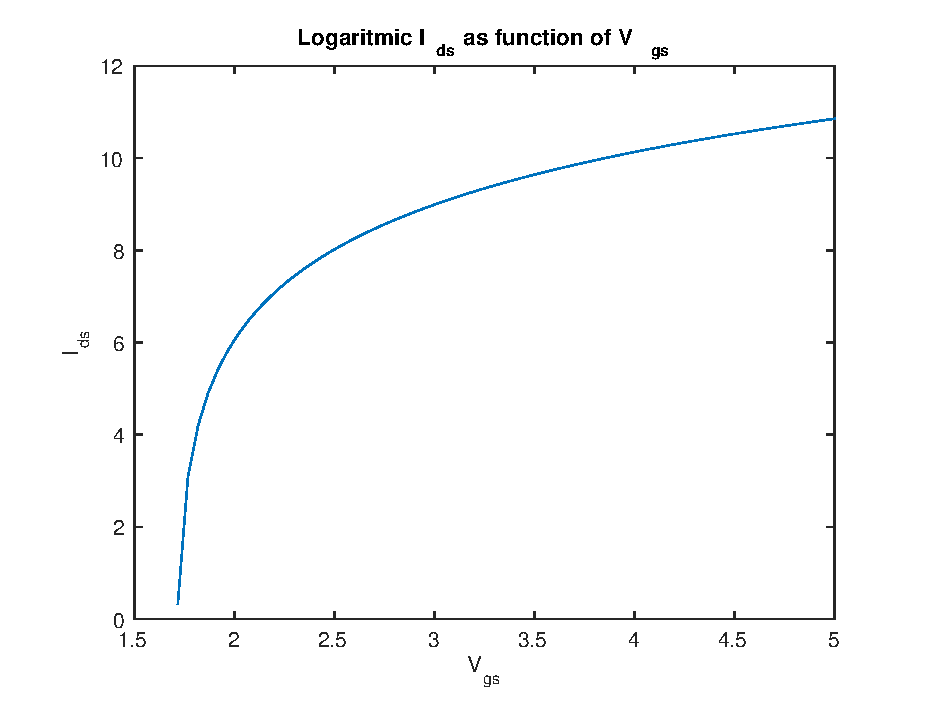
\includegraphics[scale=0.9]{task1-log.eps}
\end{figure}
\begin{figure}[ht!]
\caption{Task 2 not Matched parameters}
\centering
\includegraphics[scale=1]{task2-nomatch-eps-converted-to.pdf}
\end{figure}
\begin{figure}[ht!]
\caption{task 2 Matched parameters}
\centering
\includegraphics[scale=1]{task2-match-eps-converted-to.pdf}
\end{figure}
And nnow the logaritmic $I_{ds}$
\begin{figure}[ht!]
\caption{Task2 nMOS Not matched parameters}
\centering
\includegraphics[scale=1]{task2-nomatch-log-eps-converted-to.pdf}
\end{figure}
\begin{figure}[ht!]
\caption{Task 2 nMOSMatched parameters}
\centering
\includegraphics[scale=1]{task2-match-log-eps-converted-to.pdf}
\end{figure}
\begin{figure}[ht!]
\caption{Task 3 Resistor $I_{out}$}
\centering
\includegraphics[scale=1]{task3-eps-converted-to.pdf}
\end{figure}
\begin{figure}[ht!]
\caption{Task 4}
\centering
\includegraphics[scale=1]{task4-lin.png}
\end{figure}
Logaritmic scaling of $I_{ds}$
\begin{figure}[ht!]
\caption{task 4 log}
\centering
\includegraphics[scale=1]{task4-log-eps-converted-to.pdf}
\end{figure}
\begin{figure}[ht!]
\caption{Task 5: Circuit for measuring the cmos's}
\centering
\includegraphics[scale=0.2]{task5.png}
\end{figure}
 \begin{figure}[ht!]
\caption{task6: pMOS }
\centering
\includegraphics[scale=1]{task6.png}
\end{figure}
\begin{figure}[ht!]
\caption{Task6: pMOS logaritmic }
\centering
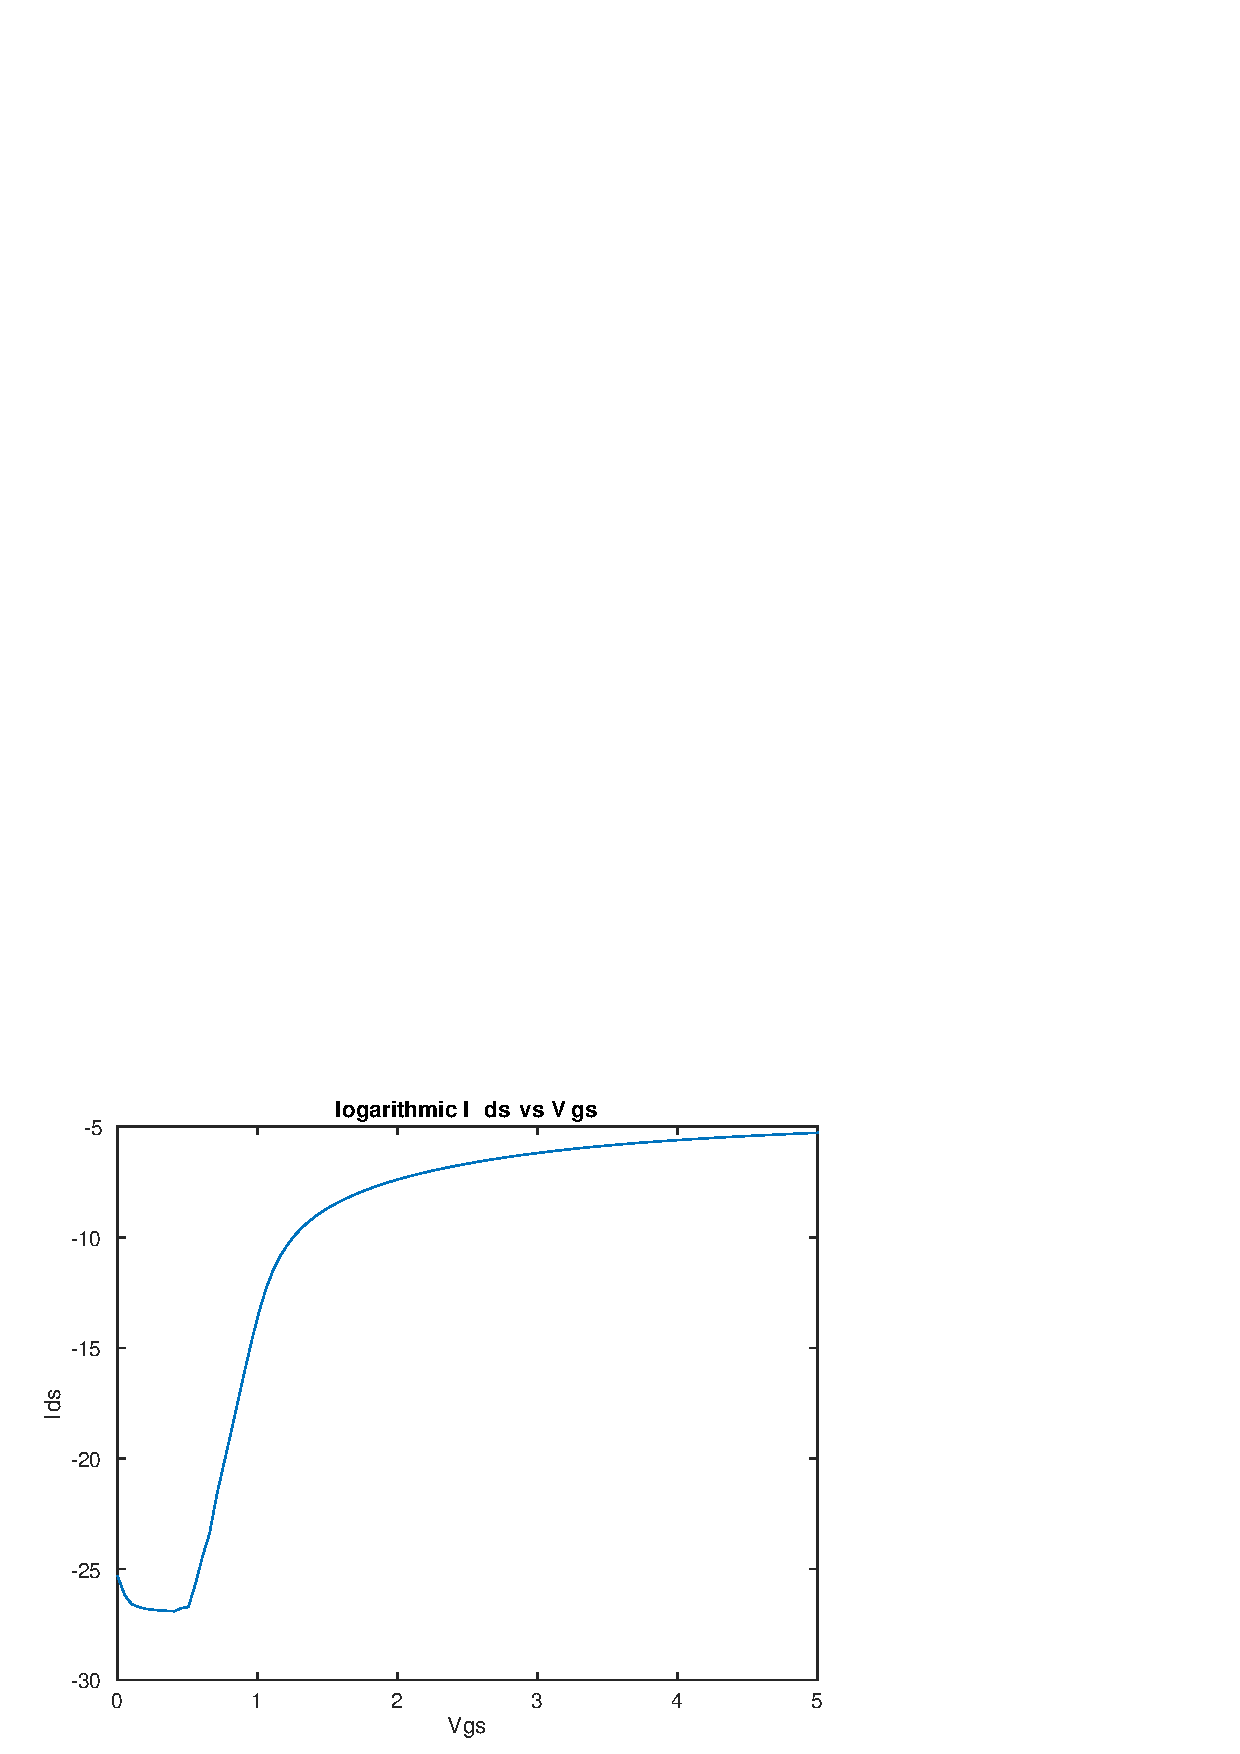
\includegraphics[scale=1]{task6log.png}
\end{figure}
\begin{figure}[ht!]
\caption{Task8: }
\centering
\includegraphics[scale=1]{task8.png}
\end{figure}
\begin{figure}[ht!]
\caption{Task10: }
\centering
\includegraphics[scale=1]{task10.png}
\end{figure}
\end{document}
